\documentclass[12pt]{article}
\usepackage{fullpage,graphicx,psfrag,url}
\usepackage[small,bf]{caption}

\usepackage{amsmath}
\usepackage{amsthm}
\usepackage{amssymb}
\usepackage{verbatim}

\setlength{\captionmargin}{30pt}

\input defs.tex
\newcommand{\sign}{\mathop{\bf sign}}

\bibliographystyle{alpha}

\title{Symbolic Subdifferentiation in Python}
\author{Maurizio Cal\'o and Jaehyun Park\\
EE 364B Project Final Report\\
Stanford University, Spring 2010-11}

\begin{document}
\maketitle

\section{Introduction}
\subsection{Motivation}
Motivated by the first two weeks of lectures, we've implemented a
Python package \verb'Subgradient-PY' (\verb'SPY') that solves
optimization problems using subgradient methods. Some features of \verb'SPY' are:

\begin{itemize}
\item The objective function and constraints need not be differentiable.
\item Due to little space usage, \verb'SPY' can be used to solve large problems.
\item \verb'SPY' can be combined with primal or dual decomposition techniques to develop distributed algorithms.
\end{itemize}


\section{A Quick Start}
\verb'SPY' can be downloaded from \url{http://www.stanford.edu/~liszt90/spy}. There is no installation package, so one can simply download the codes and unzip it to a directory named \verb'spy'.

\subsection{Example Code}
\begin{verbatim}
from spy import *
x = var('x')
y = var('y')
ex = max(x + y, 2 * x - y) + square(x)
constraints = [geq(x, y), leq(norm2([x, y]), 1)]
prob = minimize(ex, constraints)
(optval, optpoint) = prob.solve()
\end{verbatim}

\noindent Let us examine this specification line by line:

\begin{itemize}
\item The first line imports all modules from the \verb'SPY' package.
\item The second and third line declare $x$ and $y$ as the (scalar)
  optimization variables.
\item The fourth line declares an instance of the Expression class,
  corresponding to the mathematical expression: $max(x+y,2x-y)+x^2$.
\item The fifth line specifies the constraints of the optimization
  problem: $x \geq y$ and $\sqrt{x^2+y^2} \leq 1$.
\item The sixth line defines the optimization problem: ``minimize the
  given expression subject to the specified constraints.''
\item The last line solves the optimization problem using a
  subgradient method.
\end{itemize}

\noindent Printing out \verb'optval' and \verb'optpoint' gives the following:
\begin{verbatim}
-0.250040107722
{'y': -0.50654454816398864, 'x': -0.50662859414656536}
\end{verbatim}
The analytic solution is $x=y=-1/2$ with the optimal value $f^\star = -1/4$.

\section{Basics}

\subsection{Main Classes}
Along with \verb'CVX'-like library functions, \verb'SPY' implements three
important classes:
\begin{itemize}
\item Expression: Any real-valued mathematical expression is an object
of Expression type. It can contain variables whose values are not
predetermined.
\item Constraint: A constraint is an inequality of the form
$(\mbox{convex}) \le (\mbox{concave})$ or an equality of the form
$(\mbox{affine}) = (\mbox{affine})$.
\item (Optimization) Problem: A problem is a triplet of the form (minimize/maximize, objective, list of constraints).
\end{itemize}

The essential part of the project is to compute subgradients correctly
and efficiently, since all other methods rely heavily on subgradients.



\subsection{Declaring Variables}
In the current version of the \verb'SPY', one can declare a variable using the following command.
\begin{verbatim}
x = var('x')
\end{verbatim}
The meaning should be clear from the syntax; the line above declares a
variable whose name is \verb'x' without a value assigned to it. The object \verb'x' is a symbolic link to the variable with the identifier string \verb,'x',.

\subsection{Forming an Expression}
With variables, it is possible to form more complicated expressions. To
provide a clean interface to the user, we have overloaded operators as
well as some of the Python built-in functions. This allows users to form
expressions in a more natural way. For instance, the following line will create an expression named \verb'ex'.
\begin{verbatim}
ex = abs(x-3)+exp(x)
\end{verbatim}
The expression above corresponds to a mathematical expression
$|x-3|+e^x$. It should be noted that \verb'SPY' does not attempt to
simplify a given expression, nor does it immediately compute the value of
a newly formed expressions. All computations are done lazily; the
values will be computed only when the \verb'get_value' method is called on
it. Internally, the expression is stored as a tree shown in the following diagram:


\begin{center}
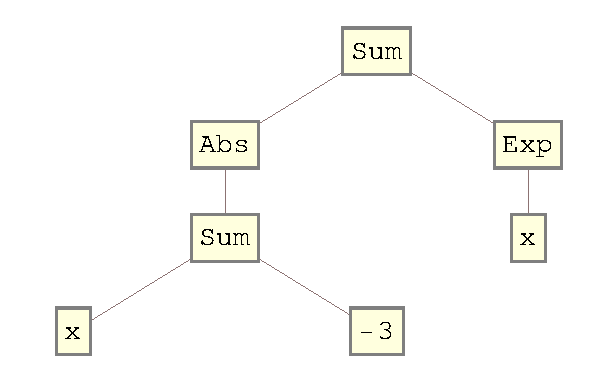
\includegraphics[width=0.45\textwidth]{expr}
\end{center}

(For a list of library functions, see section 4.4)

\subsection{Retrieving Values or Subgradients}
Because the values of variables in an expression is not predetermined, a user needs to specify them manually in order to retrieve the actual value or a subgradient of the expression. The values of the variables are not passed in as a list of numbers as one might expect. Rather, the values are passed as a dictionary that maps the name of variables to their values. The benefit of this design is that one can readily access the value of a variable by its name.

\begin{verbatim}
varmap = {'x': 1.5, 'y': -2}
val = ex.get_value(varmap)
g = ex.subgrad(varmap)
\end{verbatim}

The code above will evaluate the expression \verb'ex' at $x=1.5$ and $y=-2$, and store the (scalar-valued) result in \verb'val'. Note that the argument to the \verb'get_value' method is a dictionary. The next line computes a subgradient of \verb'ex' evaluated at the same point, storing the result into \verb'g'. The data type of \verb'g' is the same as that of \verb'varmap'. For these methods to work correctly, users need to specify the values of all the variables present in the expression. Otherwise, \verb'nan' will be returned.

The subgradient computation, as mentioned above, is the most crucial part of this project. This feature has been tested by multiple scripts that solve simple optimization problems. Also, whenever a new library function is added, a unit test is implemented in order to ensure that the functions behave as expected.

\subsection{Specifying Constraints}
One can use \verb'leq', \verb'eq', or \verb'geq' (corresponding to 
``$\le$'', ``$==$'', and  ``$\ge$'' respectively) to construct a constraint
object. Example:

\begin{verbatim}
cons = leq(norm2([x1, x2]), y)
\end{verbatim}

At construction time, \verb'SPY' automatically checks whether inequalities
and equalities follow the DCP ruleset. Constraints should be of the form
$(\mbox{convex}) \le (\mbox{concave})$ or 
$(\mbox{affine}) = (\mbox{affine})$ in the case of equality constraints.

(One other important feature of the constraint class is the cutting plane
method. This method returns a deep cutting plane whenever a constraint is
violated. Mention an example..)


\subsection{Solving Optimization Problems}
One can solve convex optimization problems using the following syntax:
\begin{verbatim}
myprob = minimize(ex, [cons1, cons2])
(optval, optpoint) = myprob.solve()
\end{verbatim}
The lines above minimizes the expression \verb'ex' subject to two constraints
\verb'cons1' and \verb'cons2' using the subgradient method. As a result,
the optimal point as well as the objective value at that point will be
returned. Advanced users can specify the step size rule used by the
method.

\section{Technical Details}

\subsection{Computation of Subgradients}
Subgradient computations are done recursively, and the procedure is
analogous to the chain rule for differentiable functions. 
For each library function (See Section 4.4), we've implemented a method that computes 
its subgradient at a given point. 
Subgradients of more complicated expressions can be computed 
using the composition rule \cite{subg}:
\begin{itemize}
\item Let $f(x) = h(f_1(x), \ldots, f_k(x))$ with $h$ convex non-decreasing,
  $f_i$ convex.
\item Find $c \in \partial h(f_1(x), \ldots, f_k(x))$,  $g_i \in \partial
  f_i(x)$
\item Then, $g = c_1 g_1 + c_2 g_2 + \cdots + c_k g_k$ is a subgradient of $f$ at $x$.
\end{itemize}


\subsection{DCP ruleset}
Whenever a constraint is specified, the constraints class automatically checks whether inequalities
and equalities follow the DCP ruleset. Similarly, the problem class checks
whether the objective of the minimization (maximation) is convex (concave). This is done by applying the
general vector composition rule \cite{cvx}, using the monotonicity and
convexity properties of the atomic functions.


\subsection{Subgradient Method}
The \verb'prob.solve()' function implements a subgradient method, which is similar to gradient descent methods for minimizing differentiable functions.

\begin{itemize}
\item At $x^{(k)}$, find $g^{(k)} \in \partial f(x^{(k)})$.
\item Set the next point as $x^{(k+1)}:=x^{(k)}-\alpha_kg^{(k)}$, where $\alpha_k$ is $k$-th step size.
\end{itemize}

Talk about step size rule, etc..

\subsection{Library Functions}
The following list contains the functions that are implemented in the current version of \verb'SPY'. For more details, please refer to the \verb'CVX' user guide \cite{guide}.
\begin{itemize}
\item \verb'abs', \verb'max', \verb'min', \verb'pos', \verb'power', \verb'power_pos'
\item \verb'exp', \verb'log', \verb'log_sum_exp', \verb'rel_entr'
\item \verb'norm1', \verb'norm2', \verb'berhu', \verb'huber'
\item \verb'square', \verb'square_pos', \verb'sqrt', \verb'geo_mean', \verb'quad_over_lin'
\end{itemize}
Functions that take a vector as an argument (e.g. \verb'max', \verb'geom_mean') currently take a list of scalars as an input, since we don't have vector-valued expressions yet.

\section{Limitations}

\begin{itemize}
\item \verb'SPY' does not work well with equality constraints (yet).
\item Convergence behavior depends on the step sizes, so it is up to users to give a ``right'' step size rule.
\item Currently, \verb'SPY' cannot detect if the given problem is unbounded. Extending \verb'SPY' to detect unboundedness will be a great deal of work, but it will be useful.
\item Extension (tentative): After we have a basic system supporting all the features above, we will extend the code to support vectors and matrices.
\end{itemize}




\begin{thebibliography}{99}
\bibitem{subg} S. Boyd, \emph{Subgradients}, EE 364B Lecture Slides, 2011.
\bibitem{guide} M. Grant and S. Boyd, \verb'cvx' \emph{Users' Guide}, 2011.
\bibitem{cvx} S. Boyd, \emph{Convex Functions}, EE 364A Lecture Slides, 2011.
\end{thebibliography}

\end{document}

